\documentclass{article}
\usepackage[utf8]{inputenc}
\usepackage[table]{xcolor}
\usepackage{graphicx}
\usepackage[T1]{fontenc}
\usepackage{imakeidx}
\usepackage{etoolbox}
\usepackage{tabularx}
\usepackage{booktabs}
\usepackage{outlines}
\usepackage{forloop}
\usepackage{pgfgantt}
\usepackage{comment}
\usepackage[normalem]{ulem}
\usepackage{hhline}
\usepackage{xcolor,colortbl}
\usepackage[dvipsnames]{xcolor}
\makeindex[name=Alphabetical,title={Alphabetical Index},columns=1]
\makeindex[name=Test-Cases,title={Index of Test Cases},columns=1]

\makeatletter
\def\@idxitem{\par\addvspace{20\p@ \@plus 2.5\p@ \@minus 1.5\p@}\hangindent 40\p@}
\def\subitem{\par\hangindent 40\p@ \hspace*{20\p@}}
\def\subsubitem{\par\hangindent 40\p@ \hspace*{30\p@}}
\renewcommand\indexspace{\par\addvspace{10\p@ \@plus 5\p@ \@minus 3\p@}}
\patchcmd\theindex{\indexname}{\indexname\vspace{14pt}}{}{}
\makeatother

\newcounter{loopcntr}
\newcommand{\rpt}[2][1]{%
  \forloop{loopcntr}{0}{\value{loopcntr}<#1}{#2}%
}
\newcommand{\on}[1][1]{
  \forloop{loopcntr}{0}{\value{loopcntr}<#1}{&\cellcolor{gray}}
}
\newcommand{\off}[1][1]{
  \forloop{loopcntr}{0}{\value{loopcntr}<#1}{&}
}

\indexsetup{othercode=\large}
\begin{comment}
Above is to make index font size large
\end{comment}

\begin{comment}


- Preface
- Introduction
    - Intentions
- Glossary
- Test cases (based off basic requirements) crossreference to 
X 1.0 - Testing Receive emails (Karsten)
X 1.1 - Testing Compose/Send/forward/reply emails
 1.1.0 - Testing Compose (Nikita)
X 1.1.1 - Testing Send (Artin)
 1.1.2 - Testing Forward (Phillip)
X 1.1.3 - Testing Reply (Karsten)
 1.2 - Testing Mark emails as Read / Unread (Nikita)
X 1.3 - Testing Delete emails (Artin)
 1.4 - Testing Blacklist (Phillip)
X 1.5 - Testing Signup/Login/Logout & Multiple Logins
X 1.5.0 - Testing Signup (Karsten)
 1.5.1 - Testing Login (Nikita)
X 1.5.1.0 - Testing valid email (Artin)
 1.5.2 - Testing Logout (Phillip)
X 1.5.3 - Forgot Password (Karsten)
 1.5.4 - Testing Multiple Logins (Nikita)
X 1.6 - Testing Attachments 
 1.6.0 - Testing picture attachments (Artin)
 1.6.1 - Testing file attachments (Phillip) 
 
Måske? hehe
 1.7 - Testing database 
 1.7.0 - Testing security
 1.7.1 - Load testing

Index
Testing Index

\end{comment}


\title{Test Plan - Softwareteknologi} % Sets article title
\author{Artin Ghalamkary - (AU677595) \and Karsten Bak Malle - (AU644054) \and Nikita Svanholm Alsøer - (AU639436) \and Phillip Ravn Boe Jensen - (AU681033)}% Sets authors name
\date{19-11-2021}

\begin{document}

\maketitle
\section*{Preface} \index[Alphabetical]{Preface}
The test plan include documentation such as a description of our test plan and how they are gonna cover the email clients functionalities, which is documented using test cases. This specific test plan may not contain every detail or capture every test detail of our mail clients behaviour and feature. The results from the tests may be included in a future version of the test plan or be featured in another document.

\section*{Introduction} \index[Alphabetical]{Introduction}

The purpose of this test plan is to give the user a easily understandable view of how we are testing our software through varying test cases to ensure a solid product. Since the email client is a product that consists of different layers of software, it has been a primary to fully test all functionalities and depths of the software. 
\subsection*{Intentions} \index[Alphabetical]{Intentions}

Going slightly more into the details and technicalities, for the sake of the customer, if more specifics are wanted. To ensure $100\%$ of coverage of our software through test cases, we have chosen to implement and take inspiration from Q4 and the different test cases originating from it, such as performance, load, stress, reliability, compatibility, etc.. We will not be going into depth, with these terms, but we thought it might be relevant for the customer to be introduces to these terms, as well as to the fact that we are primarily testing through the usage of black-box testing, with the help of, and by reusing, Django frameworks' premade testing functions.
\newline However, this test-plan has the intention of introducing the customer to the different test cases, in an abstract manner, hence no specific code or actual testing implementation will be shown here, only the abstract process of the test process.

\section*{Glossary} \index[Alphabetical]{Glossary}

\begin{enumerate}
    \item \textbf{Black-box:}\index[Alphabetical]{Black-box} Black-box testing is a software testing method in which the internal structure/design/implementation of the product being tested \textbf{is not} known to the tester.
    \item \textbf{White-box:}\index[Alphabetical]{White-box} White-box testing is a software testing method in which the internal structure/design/implementation of the product being tested \textbf{is} known to the tester.
    \item \textbf{Q4:}\index[Alphabetical]{Q4} Q4 (Quadrant 4 of the agile testing quadrants) is the technology facing tests with focus on performance, load, stress, etc. Special tools are often used for these tests along with automation testing.
    \item \textbf{T.B.D:}\index[Alphabetical]{T.B.D} Acronym for "To Be Determined". 
    \item \textbf{Performance testing:}\index[Alphabetical]{Performance testing} is a software testing process mainly used to identify and eliminate the performance bottlenecks in the software application.
    \item \textbf{Boundary value analysis*}\index[Alphabetical]{Boundary value analysis} bva is a boundary value analysis, which is a type of Black-box testing that focuses on errors at the boundaries of an input domain.
\end{enumerate}

\newpage
\section*{Test Cases}\index[Alphabetical]{Test Cases}
\begin{table}[h] 
\hspace{-102pt} \vspace{-4cm}
\begin{tabular}{|l|c|c|c|c|c|c|} 
\hline
\textbf{Test Case ID}     & \begin{tabular}[c]{@{}c@{}}Test Case \\Descriptions\end{tabular}                                                                                                                                          & Test Steps                                                                                                                                                                                                                                                       & Test Data                                                                                                                                                                                               & Expected Results                                                                                                                                                                                & \begin{tabular}[c]{@{}c@{}}Actual \\Results\end{tabular} & Pass/Fail  \\ 
\hline \index[Test-Cases]{\underline{Receive: \textbf{TU1.0}}}
\textbf{TU1.0}            & \begin{tabular}[c]{@{}c@{}}Checks if \\user receives \\valid emails\end{tabular}                                                                                                                          & \begin{tabular}[c]{@{}c@{}}After login,\\Go to~inbox, \\check if \\expected \\emails appear\end{tabular}                                                                                                                                                         & \begin{tabular}[c]{@{}c@{}}Expected\\Email == Received\\Email\end{tabular}                                                                                                                              & \begin{tabular}[c]{@{}c@{}}User should see \\expected emails\end{tabular}                                                                                                                       & T.B.D                                                    & T.B.D      \\ 
\hline 
\textbf{TU1.1}            & \multicolumn{6}{c|}{{\cellcolor[rgb]{0.435,0.553,0.929}}\uline{\textcolor{white}{Compose/Send/forward/reply emails }}}                                                                                                                                                                                                                                                                                                                                                                                                                                                                                                                                                                                                                                                                                                                                                                                                                                           \\ 
\hline \index[Test-Cases]{\underline{Compose: \textbf{TU1.1.0}}}
\textbf{TU1.1.0}          & \begin{tabular}[c]{@{}c@{}}Checks if \\ \textbf{compose } \\ and\textbf{ send} \\ works as \\intended\end{tabular}                                                                                                 & \begin{tabular}[c]{@{}c@{}}After login, go \\to~\textbf{compose}, \\fill out \\necessary \\information, \\check if valid\\email, click the \\\textbf{send~}button, \\check if~send \\email has correct \\information~~\end{tabular}                              & \begin{tabular}[c]{@{}c@{}}First test:\\to=='test@gmail.com',\\Subject == 'test', \\message == 'test', \\\\Second test:\\to=='test!!!gmail.com',\\Subject == 'test', \\message == 'test',~\end{tabular} & \begin{tabular}[c]{@{}c@{}}First test should\\send and be~\\received with \\correct\\information\\\\Second test\\should not send\end{tabular}                                                   & T.B.D                                                    & T.B.D      \\ 
\hline \index[Test-Cases]{\underline{Forward: \textbf{TU1.1.1}}}
\textbf{TU1.1.1}          & \begin{tabular}[c]{@{}c@{}}Checks if\\\textbf{forward}\\works as\\intended\end{tabular}                                                                                                                   & \begin{tabular}[c]{@{}c@{}}After login,\\go to compose,\\click on \textbf{forward},\\select\\email-address to\\forward it to,\\send, check\\if forwarded\\email has correct\\information\end{tabular}                                                            & \begin{tabular}[c]{@{}c@{}}sender.ForwardedEmail \\==~\\receiver.ReceivedEmail\end{tabular}                                                                                                             & \begin{tabular}[c]{@{}c@{}}User that's \\receiving should\\see the forwarded\\email in their inbox\end{tabular}                                                                                 & T.B.D                                                    & T.B.D      \\ 
\hline \index[Test-Cases]{\underline{Reply: \textbf{TU1.1.2}}}
\textbf{\textbf{TU1.1.2}} & \begin{tabular}[c]{@{}c@{}}Checks if~\\\textbf{reply }works\\as intended\end{tabular}                                                                                                                     & \begin{tabular}[c]{@{}c@{}}After login, \\go to inbox,\\click the \textbf{reply}\\button on the\\desired email\end{tabular}                                                                                                                                      & \begin{tabular}[c]{@{}c@{}}To:'email-address'\\==\\ClickedEmail:'\\email-address'\end{tabular}                                                                                                          & \begin{tabular}[c]{@{}c@{}}User should see\\compose~screen\\with email-address\\~of the desired \\email inserted as~\\receiver\end{tabular}                                                     & T.B.D                                                    & T.B.D      \\ 
\hline \index[Test-Cases]{\underline{Mark As Read/Unread: \textbf{TU1.2}}}
\textbf{TU1.2}            & \begin{tabular}[c]{@{}c@{}}Check~\\marked\\emails as\\\textbf{read},~\\check \\unmarked~\\emails as~\\\textbf{unread}\end{tabular}                                                                        & \begin{tabular}[c]{@{}c@{}}After login,\\go to inbox,\\click mark email\\as \textbf{read}, click\\unmark to set\\email as \textbf{unread}\end{tabular}                                                                                                           &                                                                                                                                                                                                         & \begin{tabular}[c]{@{}c@{}}User should see\\chosen email~\\change to read\\and then back \\to unread\end{tabular}                                                                               & T.B.D                                                    & T.B.D      \\ 
\hline

\end{tabular}
\end{table}

\newpage

\begin{table}[h] 
\hspace{-111pt} \vspace{-16cm}
\begin{tabular}{|l|c|c|c|c|c|c|} 
\hline
\textbf{Test Case ID}     & \begin{tabular}[c]{@{}c@{}}Test Case \\Descriptions\end{tabular}                                                                                                                                          & Test Steps                                                                                                                                                                                                                                                       & Test Data                                                                                                                                                                                               & Expected Results                                                                                                                                                                                & \begin{tabular}[c]{@{}c@{}}Actual \\Results\end{tabular} & Pass/Fail  \\ 
\hline \index[Test-Cases]{\underline{Delete: \textbf{TU1.3}}}
\textbf{TU1.3}            & \begin{tabular}[c]{@{}c@{}}Check if\\\textbf{delete email}\\works as\\intended\end{tabular}                                                                                                               & \begin{tabular}[c]{@{}c@{}}After login,\\go to inbox,~\\choose the~\\desired email to\\delete and click\\the \textbf{delete} button\end{tabular}                                                                                                                 &                                                                                                                                                                                                         & \begin{tabular}[c]{@{}c@{}}Chosen email\\should be\\deleted\end{tabular}                                                                                                                        & T.B.D                                                    & T.B.D      \\ 
\hline \index[Test-Cases]{\underline{Blacklist: \textbf{TU1.4}}}
\textbf{TU1.4}            & \begin{tabular}[c]{@{}c@{}}Check that\\\textbf{blacklist}\\correctly\\seperates\\chosen mail,\\mail-address\\into another\\folder\end{tabular}                                                            & \begin{tabular}[c]{@{}c@{}}After login,\\go to inbox,\\select email or \\email-address,\\click \textbf{blacklist }\\button\end{tabular}                                                                                                                          & \begin{tabular}[c]{@{}c@{}}~ ~inbox[email.blacklisted] \\== \\not found \\\&\& \\~blacklist[email.blacklisted] \\== \\found\end{tabular}                                                                & \begin{tabular}[c]{@{}c@{}}User should see\\the email/emails\\from the specified\\email-address\\gone from their\\inbox, and see\\it/them in the\\blacklist folder\end{tabular}                 & T.B.D                                                    & T.B.D      \\ 

\textbf{TU1.5}            & \multicolumn{6}{c|}{{\cellcolor[rgb]{0.435,0.553,0.929}}\uline{\textcolor{white}{Signup/Login/Logout \& Multiple Logins }}}                                                                                                                                                                                                                                                                                                                                                                                                                                                                                                                                                                                                                                                                                                                                                                                                                                      \\ 
\hline \index[Test-Cases]{\underline{Sign Up: \textbf{TU1.5.0}}}
\textbf{TU1.5.0}          & \begin{tabular}[c]{@{}c@{}}Check if \\\textbf{sign up~}\\works \\resulting \\in creation \\of new \\email account\end{tabular}                                                                            & \begin{tabular}[c]{@{}c@{}}Go to login,\\click \textbf{sign up}\\button, fill out\\the necessary\\information,\\pick a unique\\email-address\\and password,\\then login to\\the new email\\account\end{tabular}                                                  & \begin{tabular}[c]{@{}c@{}}NewEmailAddress\\!=\\StoredEmailAddress\end{tabular}                                                                                                                         & \begin{tabular}[c]{@{}c@{}}User should be\\signed in on the\\new email account\\assuming valid\\information is~\\given\end{tabular}                                                             & T.B.D                                                    & T.B.D      \\ 
\hline \index[Test-Cases]{\underline{Login: \textbf{TU1.5.1}}}
\textbf{TU1.5.1}          & \begin{tabular}[c]{@{}c@{}}Check \textbf{login }\\with valid \\username \\and \\password, \\check\textbf{ login }\\with invalid \\username, \\check \textbf{login }\\with invalid \\password\end{tabular} & \begin{tabular}[c]{@{}c@{}}Go to \textbf{login},\\enter valid\\username\\and password,\\click login button,\\logout,\\enter invalid\\username\\and valid\\password,~\\attempt login,\\enter valid\\username,\\and invalid\\password,\\attempt login\end{tabular} & \begin{tabular}[c]{@{}c@{}}Email.LoggedIn == true,\\Email.LoggedIn == false,\\Email.LoggedIn == false\end{tabular}                                                                                      & \begin{tabular}[c]{@{}c@{}}User should be\\logged into the\\email client, then\\after logging out,\\user should fail\\both attempts at\\login with invalid\\username and\\password\end{tabular} & T.B.D                                                    & T.B.D      \\ 
\hline

\end{tabular}
\end{table}

\newpage

\begin{table}[h] 
\hspace{-112pt} \vspace{-16cm}
\begin{tabular}{|l|c|c|c|c|c|c|} 
\hline
\textbf{Test Case ID}     & \begin{tabular}[c]{@{}c@{}}Test Case \\Descriptions\end{tabular}                                                                                                                                          & Test Steps                                                                                                                                                                                                                                                       & Test Data                                                                                                                                                                                               & Expected Results                                                                                                                                                                                & \begin{tabular}[c]{@{}c@{}}Actual \\Results\end{tabular} & Pass/Fail  \\ 
\hline \index[Test-Cases]{\underline{Logout: \textbf{TU1.5.2}}}
\textbf{TU1.5.2}          & \begin{tabular}[c]{@{}c@{}}Check if\\user correctly\\logs out\\when\textbf{ logout}\\button\\is clicked\end{tabular}                                                                                      & \begin{tabular}[c]{@{}c@{}}Go to login,\\enter valid\\username\\and password,\\click login button,\\then click \textbf{logout}\\button\end{tabular}                                                                                                              & Email.LoggedIn == false                                                                                                                                                                                 & \begin{tabular}[c]{@{}c@{}}User should be\\logged out of\\the email client,\\with the selected\\email account\end{tabular}                                                                      & T.B.D                                                    & T.B.D      \\ 
\hline \index[Test-Cases]{\underline{Forgot Password: \textbf{TU1.5.3}}}
\textbf{TU1.5.3}          & \begin{tabular}[c]{@{}c@{}}Check if\\\textbf{forgot}\\\textbf{password}\\requires\\security\\check,~\\then check\\if \textbf{forgot}\\\textbf{password}\\overrides\\the forgotten\\password\end{tabular}  & \begin{tabular}[c]{@{}c@{}}Go to login,\\click \textbf{forgot}\\\textbf{password} \\button, \\complete~\\security steps,\\attempt login\\with old\\password,\\fail, then login\\with new\\password\end{tabular}                                                  & \begin{tabular}[c]{@{}c@{}}SecurityComplete == true,\\LoginOld == false,\\LoginNew == true\end{tabular}                                                                                                 & \begin{tabular}[c]{@{}c@{}}After completing\\security steps\\user should be\\able to login with\\new password\\and not old~\\password\end{tabular}                                              & T.B.D                                                    & T.B.D      \\ 
\hline \index[Test-Cases]{\underline{Multiple Logins: \textbf{TU1.5.4}}}
\textbf{TU1.5.4}          & \begin{tabular}[c]{@{}c@{}}Check if\\the login\\page allows\\to log in\\simultaneously\\with different\\credentials in\\a different\\browser\end{tabular}                                                 & \begin{tabular}[c]{@{}c@{}}Go to login,\\login as user1\\with user1\\credentials, open\\new browser,\\go to login,\\login as user2\\with user2\\credentials\end{tabular}                                                                                         & \begin{tabular}[c]{@{}c@{}}User1.LoggedIn == true\\User2.LoggedIn == true\end{tabular}                                                                                                                  & \begin{tabular}[c]{@{}c@{}}User1 and user2\\should both be\\logged into the\\email client at\\the same time,\\as long as they\\are logged in on\\different browsers\end{tabular}                & T.B.D                                                    & T.B.D      \\ 
\hline 
\textbf{TU1.6}            & \multicolumn{6}{c|}{{\cellcolor[rgb]{0.435,0.553,0.929}}\uline{\textcolor{white}{Attachments }}}                                                                                                                                                                                                                                                                                                                                                                                                                                                                                                                                                                                                                                                                                                                                                                                                                                                                 \\ 
\hline \index[Test-Cases]{\underline{Picture Attachment: \textbf{TU1.6.0}}}
\textbf{TU1.6.0}          & \begin{tabular}[c]{@{}c@{}}Check if\\email can\\send with\\\textbf{picture}\\\textbf{attachment}\end{tabular}                                                                                             & \begin{tabular}[c]{@{}c@{}}After login,\\go to compose,\\fill out necessary\\information,~\\choose \textbf{picture}\\to attach, \\click send\end{tabular}                                                                                                        & \begin{tabular}[c]{@{}c@{}}ReceivedMail\\==\\SendMailWithAttachment\\Attachment: jpg/png\end{tabular}                                                                                                   & \begin{tabular}[c]{@{}c@{}}Mail sent with\\attached picture\end{tabular}                                                                                                                        & T.B.D                                                    & T.B.D      \\ 
\hline \index[Test-Cases]{\underline{File Attachment: \textbf{TU1.6.1}}}
\textbf{TU1.6.1}          & \begin{tabular}[c]{@{}c@{}}Check if \\email can\\send with\\\textbf{file }\\\textbf{attachment}\end{tabular}                                                                                              & \begin{tabular}[c]{@{}c@{}}After login,\\go to compose,\\fill out necessary\\information,~\\choose\textbf{ file}\\to attach, \\click send\end{tabular}                                                                                                           & \begin{tabular}[c]{@{}c@{}}ReceivedMail\\==\\SendMailWithAttachment\\Attachment: filetype\end{tabular}                                                                                                  & \begin{tabular}[c]{@{}c@{}}Mail sent with\\attached files\end{tabular}                                                                                                                          & T.B.D                                                    & T.B.D      \\
\hline
\end{tabular}
\end{table}

\newpage
\newpage

\definecolor{cornflowerblue}{rgb}{0.39, 0.58, 0.93}

\vspace{5 mm}

\centerline{
\begin{tabular}{| c |}
 \hline
 User requirements\\
 \hline 
 \rowcolor{cornflowerblue}
 1. Mail client should be able to display\index[Functions]{Display}, send\index[Functions]{Send}, and receive\index[Functions]{Receive} emails as well as let the user be able & \rowcolor{cornflowerblue} to reply\index[Functions]{Reply} and forward\index[Functions]{Forward} the emails received through the selected server. \\
 \hline
 \rowcolor{cornflowerblue}
 2. Mail client should provide the user the opportunity to login\index[Functions]{Login} to their personal email\\
 \hline
 \rowcolor{cornflowerblue}
 3. The user should be able to blacklist\index[Functions]{Blacklist} any email\\
 \hline
 \rowcolor{cornflowerblue}
 4. The user should be able to login to multiple emails\index[Functions]{Online - multiple emails} at the same time\\
 \hline
 \rowcolor{cornflowerblue}
 5. The user should be able to delete\index[Functions]{Delete} any email\\
 \hline
 \rowcolor{cornflowerblue}
 6. The user should be able to mark emails as read/unread\index[Functions]{Mark - read/unread}\\
 \hline
 \rowcolor{cornflowerblue}
 7. The user should be able attach files and pictures\index[Functions]{Attach files/pictures} to their emails\\
 \hline
 \rowcolor{cornflowerblue}
 8. The user should be able to compose\index[Functions]{Compose} a email\\

\end{tabular}
}

\vspace{5 mm}

\begin{center}
\begin{tabular}{| c |}
 \hline
 Nonfunctional requirements\\
 \hline 
 \rowcolor{cornflowerblue}
 1. Limited database \\
 \hline
 \rowcolor{cornflowerblue}
 2. Interval of email fetching\\
 \hline
 \rowcolor{cornflowerblue}
 3. Mail client will be driven by localhost\\
 \hline
 \rowcolor{cornflowerblue}
 4. Mail client downtime\\
 \hline
 \rowcolor{cornflowerblue}
 5. File attachment size constraint\\
 \hline
\end{tabular}
\end{center}
The above requirements have been taken from our \textbf{System-requirements} report. The first table, \textbf{User requirements} is the area of focus for testing, this is where the implementation of Black-box, White-box and Q4 testing will occur. The second table, \textbf{Nonfunctional requirements} will not be tested. 

\section*{Testing approach}\index[Alphabetical]{Testing approach}
It was mentioned at the beginning of the document that we would use different types of testing methods, such as Black-box testing and test method from Q4 testing. This section will describe what the different test methods are, and we will come with examples of which test cases uses which testing method. It should be mentioned that more test methods, other than the two test methods mentioned above, will be used.
\newline
Starting with Black-box testing and White-box testing. Black-box testing is a software testing method in which the internal structure/design/implementation of the product being tested \textbf{is not} known to the tester. White-box testing is a software testing method in which the internal structure/design/implementation of the product being tested \textbf{is} known to the tester. For a visual understanding, see the figure underneath that describes Black-box and White-box testing.
\begin{center}
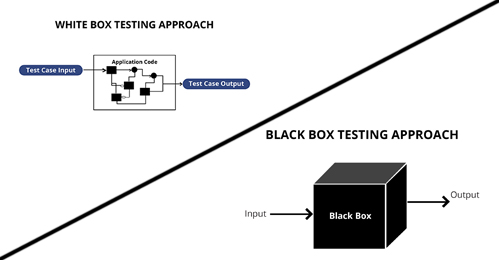
\includegraphics[width = \linewidth]{BlackboxvsWhitebox.jpg} 
\end{center}
The other types of testing is Q4 testing. Q4 (Quadrant 4 of the agile testing quadrants) is the technology facing tests with focus on performance, load, stress, etc. Special tools are often used for these tests along with automation testing.
\item \textbf{T.B.D:}\index[Alphabetical]{T.B.D} Acronym for "To Be Determined". An example of queue testing would be performance test, and we will use performance test throughout most test cases, but an example would be test case TU1.1.0. Another testing method we will do is bva's which is boundary value analysis, which is a type of Black-box testing that focuses on errors at the boundaries of an input domain.


\section*{Testing responsibility}\index[Alphabetical]{Testing responsibility}
It can be read from the systems requirement report that the clients functionalities and behaviour is split between frontend, middleware and backend. Each member has been assigned a role and work in the scope of that role. The testing will primarily be done together as unity, but the different members may have more expertise, when it comes to the different scopes.

\section*{Risks and Contingencies}\index[Alphabetical]{Risks and Contingencies}

A side note that is relevant to mention when talking about testing of the software, is to expect the unexpected, and how to deal with unexpected changes. With our mindset of the agile development process, the focus has always been to be prepared when faced with spontaneous changes. In the scenario of a customer wanting to fundamentally change his/her requirements, it is ideal to be able to sufficiently deal with the problem, by correctly distributing the roles and workload evenly out between all working members of the company. However, in the case of this project, the product is not very big and complex, hence the risk would most likely never scale out of proportion.
\newpage

\section*{Corrections to report}\index[Alphabetical]{Corrections to report}

\begin{center}
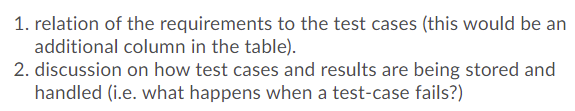
\includegraphics[width = \linewidth]{feedback_test_plan.png} 
\end{center}
\hspace{-5.3mm}\textcolor{red}{1. The following table showcases the relation between the test cases and our requirements:}
\begin{table}[h] 
\hspace{-20.3pt} \vspace{-2cm}
\arrayrulecolor{black}
\begin{tabular}{|l|c!{\color{red}\vrule}} 
\cline{1-1}\arrayrulecolor{red}\cline{2-2}
\begin{tabular}[c]{@{}l@{}}\textbf{}\\\textbf{~ ~ Test Case ID~ ~~}\\\textbf{}\end{tabular}                                                                & \textbf{\textcolor{red}{Relation of requirements to test cases}}                                                                                                   \\ 
\arrayrulecolor{black}\cline{1-1}\arrayrulecolor{red}\cline{2-2}
\begin{tabular}[c]{@{}l@{}}\textbf{\textbf{TU1.0}}\\\textbf{\textbf{}}\end{tabular}                                                                        & \textcolor{red}{Tests requirements ID 1: Display emails}                                                                                                           \\ 
\hhline{>{\arrayrulecolor{black}}|->{\arrayrulecolor{red}}-|}
\rowcolor[rgb]{0.435,0.553,0.929} \begin{tabular}[c]{@{}>{\cellcolor[rgb]{0.435,0.553,0.929}}l@{}}\textbf{\textbf{TU1.1}}\\\textbf{\textbf{}}\end{tabular} & \uline{\textcolor{white}{Compose/Send/Forward/Reply emails}}                                                                                                       \\ 
\arrayrulecolor{black}\cline{1-1}\arrayrulecolor{red}\cline{2-2}
\begin{tabular}[c]{@{}l@{}}\textbf{\textbf{}}\\\textbf{\textbf{TU1.1.0}}\\\textbf{\textbf{}}\end{tabular}                                                  & \begin{tabular}[c]{@{}c@{}}\textcolor{red}{Tests user requirements ID 8: Compose emails}\\\textcolor{red}{Tests~user requirements ID 1: Send emails}\end{tabular}  \\ 
\arrayrulecolor{black}\cline{1-1}\arrayrulecolor{red}\cline{2-2}
\begin{tabular}[c]{@{}l@{}}\textbf{\textbf{TU1.1.1}}\\\textbf{\textbf{}}\end{tabular}                                                                      & \textcolor{red}{Tests~user requirements ID 1: Forward emails}                                                                                                      \\ 
\arrayrulecolor{black}\cline{1-1}\arrayrulecolor{red}\cline{2-2}
\begin{tabular}[c]{@{}l@{}}\textbf{\textbf{TU1.1.2}}\\\textbf{\textbf{}}\end{tabular}                                                                      & \textcolor{red}{Tests~user requirements ID 1: Reply to emails}                                                                                                     \\ 
\arrayrulecolor{black}\cline{1-1}\arrayrulecolor{red}\cline{2-2}
\begin{tabular}[c]{@{}l@{}}\textbf{\textbf{TU1.2}}\\\textbf{\textbf{}}\end{tabular}                                                                        & \textcolor{red}{Tests~user requirements ID 6: Mark emails as read/unread}                                                                                          \\ 
\arrayrulecolor{black}\cline{1-1}\arrayrulecolor{red}\cline{2-2}
\begin{tabular}[c]{@{}l@{}}\textbf{TU1.3}\\\textbf{}\end{tabular}                                                                                          & \textcolor{red}{Tests~user requirements ID 5: Delete any email}                                                                                                    \\ 
\arrayrulecolor{black}\cline{1-1}\arrayrulecolor{red}\cline{2-2}
\begin{tabular}[c]{@{}l@{}}\textbf{TU1.4}\\\textbf{}\end{tabular}                                                                                          & \textcolor{red}{Tests~user requirements ID 3: Blacklist any email}                                                                                                 \\ 
\hhline{>{\arrayrulecolor{black}}|->{\arrayrulecolor{red}}-|}
\rowcolor[rgb]{0.435,0.553,0.929} \begin{tabular}[c]{@{}>{\cellcolor[rgb]{0.435,0.553,0.929}}l@{}}\textbf{TU1.5}\\\textbf{}\end{tabular}                   & \uline{\textcolor{white}{Signup/Login/Logout Multiple Logins }}                                                                                                    \\ 
\arrayrulecolor{black}\cline{1-1}\arrayrulecolor{red}\cline{2-2}
\begin{tabular}[c]{@{}l@{}}\textbf{TU1.5.0}\\\textbf{}\end{tabular}                                                                                        & \textcolor{red}{Tests~user requirements ID 2: Login to personal email}                                                                                             \\ 
\arrayrulecolor{black}\cline{1-1}\arrayrulecolor{red}\cline{2-2}
\begin{tabular}[c]{@{}l@{}}\textbf{TU1.5.1}\\\textbf{}\end{tabular}                                                                                        & \textcolor{red}{Tests~user requirements ID 2: Login to personal email}                                                                                             \\ 
\arrayrulecolor{black}\cline{1-1}\arrayrulecolor{red}\cline{2-2}
\begin{tabular}[c]{@{}l@{}}\textbf{\textbf{TU1.5.2}}\\\textbf{\textbf{}}\end{tabular}                                                                      & \textcolor{red}{Tests~user requirements ID 2: Login to personal email}                                                                                             \\ 
\arrayrulecolor{black}\cline{1-1}\arrayrulecolor{red}\cline{2-2}
\begin{tabular}[c]{@{}l@{}}\textbf{\textbf{TU1.5.3}}\\\textbf{\textbf{}}\end{tabular}                                                                      & \textcolor{red}{Tests~user requirements ID 2: Login to personal email}                                                                                             \\ 
\arrayrulecolor{black}\cline{1-1}\arrayrulecolor{red}\cline{2-2}
\begin{tabular}[c]{@{}l@{}}\textbf{\textbf{TU1.5.4}}\\\textbf{\textbf{}}\end{tabular}                                                                      & \textcolor{red}{Tests~user requirements ID 4: Login to multiple emails}                                                                                            \\ 
\hhline{>{\arrayrulecolor{black}}|->{\arrayrulecolor{red}}-|}
\rowcolor[rgb]{0.435,0.553,0.929} \begin{tabular}[c]{@{}>{\cellcolor[rgb]{0.435,0.553,0.929}}l@{}}\textbf{\textbf{TU1.6}}\\\textbf{\textbf{}}\end{tabular} & \uline{\textcolor{white}{Signup/Login/Logout Multiple Logins}}                                                                                                     \\ 
\arrayrulecolor{black}\cline{1-1}\arrayrulecolor{red}\cline{2-2}
\begin{tabular}[c]{@{}l@{}}\textbf{\textbf{\textbf{\textbf{TU1.6.0}}}}\\\textbf{\textbf{\textbf{\textbf{}}}}\end{tabular}                                  & \textcolor{red}{Tests~user requirements ID 7: attach files/pictures to emails}                                                                                     \\ 
\arrayrulecolor{black}\cline{1-1}\arrayrulecolor{red}\cline{2-2}
\begin{tabular}[c]{@{}l@{}}\textbf{\textbf{\textbf{\textbf{TU1.6.1}}}}\\\textbf{\textbf{\textbf{\textbf{}}}}\end{tabular}                                  & \textcolor{red}{Tests~user requirements ID 7: attach files/pictures to emails}                                                                                     \\
\arrayrulecolor{black}\cline{1-1}\arrayrulecolor{red}\cline{2-2}
\end{tabular}
\arrayrulecolor{black}
\end{table}
\newpage
\hspace{-5.3mm}\textcolor{red}{2. Django will create a dynamic test database that stores the values and the results from the test cases as well as destroy the test database when the tests have run. In case of test failure, there will be raised either an exception error or assertion error with information regarding it. This will be displayed in the terminal that is used to run the tests.} 


\newpage

\printindex[Alphabetical]
\printindex[Test-Cases]





\end{document}

